\chapter{Overview of CryptDB}
\label{chp:overview_cryptDB}

\section{System Architecture}

CrytpDB's architecture (Figure \ref{cryptdb_plain}) is divided into two pieces, more specific a proxy server and a database server. The proxy server is an intermediate server placed between the application server (used by the application to manage key set-up and interacting with clients) and the database server. Its purpose is to intercept queries going from the application to the database and anonymize the information of the query. By doing so, it eliminates the possibility of eavesdropping attackers to obtain any sensible information. %Kommentere at Microsoft hevder å ha brukt freq attack her.
Another vital part of the proxy server's domain is to issue queries to the database that adjusts the encryption layer (or onion layer) of the column(s) that the user has issued a query on, which will be discussed in section \ref{adjust_enc_level}. The last responsibility of the proxy server is to keep track of the users that are currently logged in using a table of active keys. CryptDB has two operational modes or principals. One for applications consisting of only one user, and another for multi-user applications. Application keys consists of both a symmetric key rooted in the users application password and a public-key pair. When logging in, the proxy derives encryption keys with the user's password as the root. These keys are used for accessing the data items that are accessible to that particular user and to encrypt new items. When the user logs out, the keys are deleted from the proxy server.

\begin{figure}[h]
	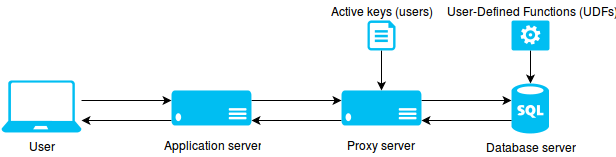
\includegraphics[scale=0.6]{CryptDB_Plain.png}
	\caption{System architecture of CryptDB interacting with a client application}
	\label{cryptdb_plain}
\end{figure}

The authors \citep{CryptDB_Main_Paper} have implemented CryptDB both with MySQL and PostgreSQL database management systems. CryptDB requires no modifying of the database system, other than adding a set of \Gls{udf}. \Gls{udf} in CryptDB allows the database to perform cryptographic operations on the encrypted data and are created using the \verb!CREATE FUNCTION! command of \gls{sql}. It also holds an encrypted table of all user-keys when in multi-user mode.

\section{SQL-Aware Encryption and the Onion Scheme}

CryptDB uses an encryption scheme called \emph{SQL-aware encryption} or \textit{onion encryption}. Basically, this means that the encryption scheme is a collection of different schemes, each providing different levels of security and computations to be executed. Data items stored using CryptDB are encrypted multiple times using these different schemes, or layers, of encryption. The result is a onion-like structure where the outer layers provide maximum security and low functionality, while the inferior layers provide less security, but more functionality.


\subsection{Random}
\Gls{random_onion} is the highest security level in CryptDB and provides the maximum security found in encryption scheme. It uses a strong block cipher such as Blowfish or \Gls{aes} in \Gls{cbc_mode} mode and a random initialization vector (IV) to ensure that the block cipher is probabilistic \citep{CryptDB_Main_Paper}. \Gls{random_onion}, being the maximum security level provided, does not allow any computation to be done on the encrypted data. In other terms, this level is a natural choice for sensitive data that are only meant to be read. When a block cipher is probabilistic, it has properties such that when encrypting the same message $m_1$ multiple times, the resulting ciphertexts are unequal. For example, given two encryptions of the same plaintext $c_1 = E_k(m_1)$ and $c_2 = E_k(m_1)$, the resulting ciphertexts are $c_1$ and $c_2$ such that $c_1 \neq c_2$. Operations supported by this scheme are \verb!SELECT!, \verb!UPDATE!, \verb!DELETE! and \verb!INSERT!.


\subsection{Deterministic}
Where \Gls{random_onion} allows no computation to be done on the encrypted data, the next layer does. \Gls{deterministic_onion} is an encryption scheme enabling the application to perform standard SQL operations such as equality checks, distinct, group by and count. By allowing these sorts of computation, the application leaks information to an adversary. In particular, it leaks which ciphertexts that decrypts to the same plaintext value. Following the previous example; if the scheme encrypted the message $m_1$ two times, the resulting ciphertexts $c_1$ and $c_2$ are such that $c_1 = c_2$. \Gls{deterministic_onion} is a deterministic scheme which, to be used correctly, should be a \Gls{prp}. In order to cope with leaking prefix equality, the authors have designed their own version of the CMC mode \cite{CryptDB_Main_Paper}.


\subsection{Order-Preserving Encoding}
Since \Gls{sql} also allows the user to compute on order relations between items, CryptDB introduces an \Gls{ope_onion} scheme \citep{CryptDB_Main_Paper}. This scheme takes starting point in a requirement where the sort order of the ciphertext matches the sort-order of the corresponding decrypted plaintexts. It also requires that the scheme reveals no other information about the plaintexts, other than the respective order. This common operation in \Gls{sql} supports order comparison, which can be used for range checks, ranking, sorting, and extracting minimum and maximum values. Popa et al. \cite{CryptDB_OPE_Encoding} introduces a scheme called \Gls{mOPE} where the main technique is mutable ciphertexts. Mutability (or malleability) is a cryptographic property allowing transformation of one ciphertext into another. More formally, given a plaintext $m_1$, it is possible to transform it into a valid encryption $f(m_1)$ by using a valid function $f$ without further knowledge of $m_1$.

\Gls{mOPE} uses a balanced binary tree for searching which contains encryptions of all the plaintext's values and a table of \Gls{ope_onion} encodings where the encoded value of a ciphertext is its path from the root to the particular node in the binary tree. If $y$ is greater than $x$, then $y$ will be located to the right of $x$ in the tree. It also uses an interactive protocol when inserting a value into the search tree, where the server and the client plays a query game. The client asks for the encrypted root node, decrypts it and determines whether the value to be inserted is smaller or larger than the root. It replies to the server with a $0$ or $1$, making the server traverse the tree to the left or right and replying with the next encrypted node. This little game continues until there are no child nodes. In order to avoid the tree being too deep, \Gls{mOPE} uses a tree-balancing transformation summary which describes operations (most of them split-and-merge operations) that are completely done by the server.

The balancing procedure ensures that the height of the tree is bounded by $\log(N)$, where $N$ is the number of encrypted values. Because both client and server needs a shared understanding of the structure of the search tree, the client computes a Merkle hash of the root of the tree. A Merkle tree is a tree where every parent node is labelled with the hash of all of its children's labels \cite{Merkle}. By performing the Merkle hash, the client is able to check whether the server behaves malicious or not (Malicious in this setting would be if the server performed other operations than the client requested) by comparing its own Merkle hash of the root with the one delivered by the server.


\subsection{Homomorphic Encryption}
Another vital part of \Gls{sql} is the ability to perform addition and multiplication. For CryptDB to be able to perform these operations, it utilizes a \Gls{hom_onion} scheme. As previously described, homomorphic encryption is a technique that enables computation on encrypted data without decrypting it first. CryptDB uses Pailler multiplication \cite{Paillier} for enabling summation operations. Pailler is originally a trapdoor mechanism based on the Composite Residuosity Class Problem which conveniently has a cryptographic property such that $HOM_k(x) * HOM_k(y) = HOM_k(x + y)$. Multiplication was not initially implemented, but has been added in later versions of CryptDB by an outside team using the El Gamal cryptosystem \cite{cryptdb_guidelines}.


\subsection{Equality Join and Order-Preserving Join}
When it comes to joining columns, two cases are supported in CryptDB. The first is the regular equality join (EQ-JOIN) between two columns, and the other is range joins (OPE-JOIN) which involves order relation checks. Ideally, the proxy server should know in advance which columns that should be allowed to be joined in order to encrypt these column with the same key. Because of the key-chaining approach where each data item is encrypted with a new key, CryptDB is in need of a separate encryption scheme in order to compute joins in a safe manner. The authors \citep{CryptDB_Main_Paper} introduces a new cryptographic primitive, \gls{join_adj}. The idea is to let the proxy server adjust the encryption keys of columns in real-time based on the observed query. \gls{join_adj} is a deterministic function, making two equal plaintexts encrypt to an identical ciphertext, and 


\subsection{Search}
In order to perform search for words in the encrypted texts, CryptDB has a scheme called SEARCH. This was an implementation of the cryptographic protocol suggested by Song et al. making it almost as secure as the \gls{random_onion} scheme \citep{CryptDB_Main_Paper}. The main idea is to split a text encrypted with SEARCH into individual keywords on a given delimiter specified by the application developer. Removal of duplicate keywords and randomly permute them are also added to enhance the security. When executing a search, the server would be given an encrypted token of the keyword, and would retrieve encrypted values matching the token. Originally, SEARCH could perform \texttt{LIKE} operations as other database systems, but in the most recent version of CryptDB's software it has been deprecated. 

% How to escape this subsection?

These different layers are wrapped into four different onion classes, namely \texttt{EQ}(Equality checks), \texttt{ORD}(Order relations), \texttt{SEARCH}(Searching) and \texttt{ADD}(Addition) as shown in Figure \ref{cryptdb_onions}. Each onion has a special purpose in means of supporting certain operations, and every data item is encrypted multiple times in each of the different onions. However, the application does not necessary maintain all of onions. There is, for example, no need for maintaining the ADD-onion if the data type is a string. 

\begin{figure}[ht]
	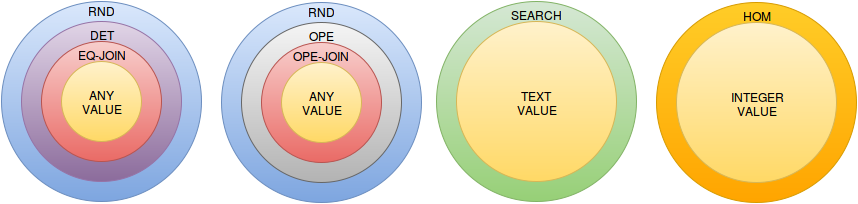
\includegraphics[scale=0.42]{Onions.png}
	\caption{From left: The EQ-onion, ORD-onion, SEARCH-onion and ADD-onion}
	\label{cryptdb_onions}
\end{figure}


\section{Adjusting the Encryption Level Based on the Query}
\label{adjust_enc_level}

A story about a spy, a castle and some walls.

\section{Threats}

\section{Security}

\section{Limitations}